\documentclass[12pt]{article}

\usepackage[spanish]{babel}
\usepackage{hyperref}
\usepackage{graphicx}
\usepackage{listings}
\usepackage{color}
\usepackage{multicol}
\usepackage{amssymb}
\spanishdecimal{.}

%% Título
\title{Matemáticas para las Ciencias Aplicadas I}

%% Fecha
\date{\today}

%% Autor
\author{Flores Morán Julieta Melina \\ Zarco Romero José Antonio}


%% Se marca el inicio del documento.
\begin{document}

%% Comando para crear el título.
\maketitle


%sección 3
\section{Problema 22}
Flores Morán Julieta Melina \\
\\
Un pequeño fabricante de electrodomésticos descubre que cuesta 9000 dólares producir 1000 tostadoras a la semana y 12000 dólares producir 1500 tostadoras a la semana.
\begin{enumerate}
\item Exprese el costo en función del número de tostadoras producidas, suponiendo que es lineal. Después, trace la gráfica.\\ 

Ya que suponemos que el costo $C$ es una función lineal del número de tostadoras $t$ de la forma $y = mx + b$, podemos escribir:

\[
	C=mt+b
\]

Utilizando los datos del problema, consideremos que conocemos los puntos (1000, 9000) y (1500, 12000). Por lo que la pendiente de la recta es

\[
	 m = \frac{\Delta {y}}{\Delta{x}} = \frac{12000-9000}{1500-1000} = \frac{3000}{500} = 6
\]

de modo que

\[
C=6t+b
\]

y su ecuación de la forma punto-pendiente $y-y_1=m(x-x_1)$, en el punto (1000, 9000) es 

\[
	C-9000=6(t-1000)
\]

o bien
\[
	C=6t+3000
\]

\[
\therefore f(t) = 6t + 3000
\]

Dicha ecuación da un posible modelo lineal, representado gráficamente como
\begin{figure}[h!]
\centering
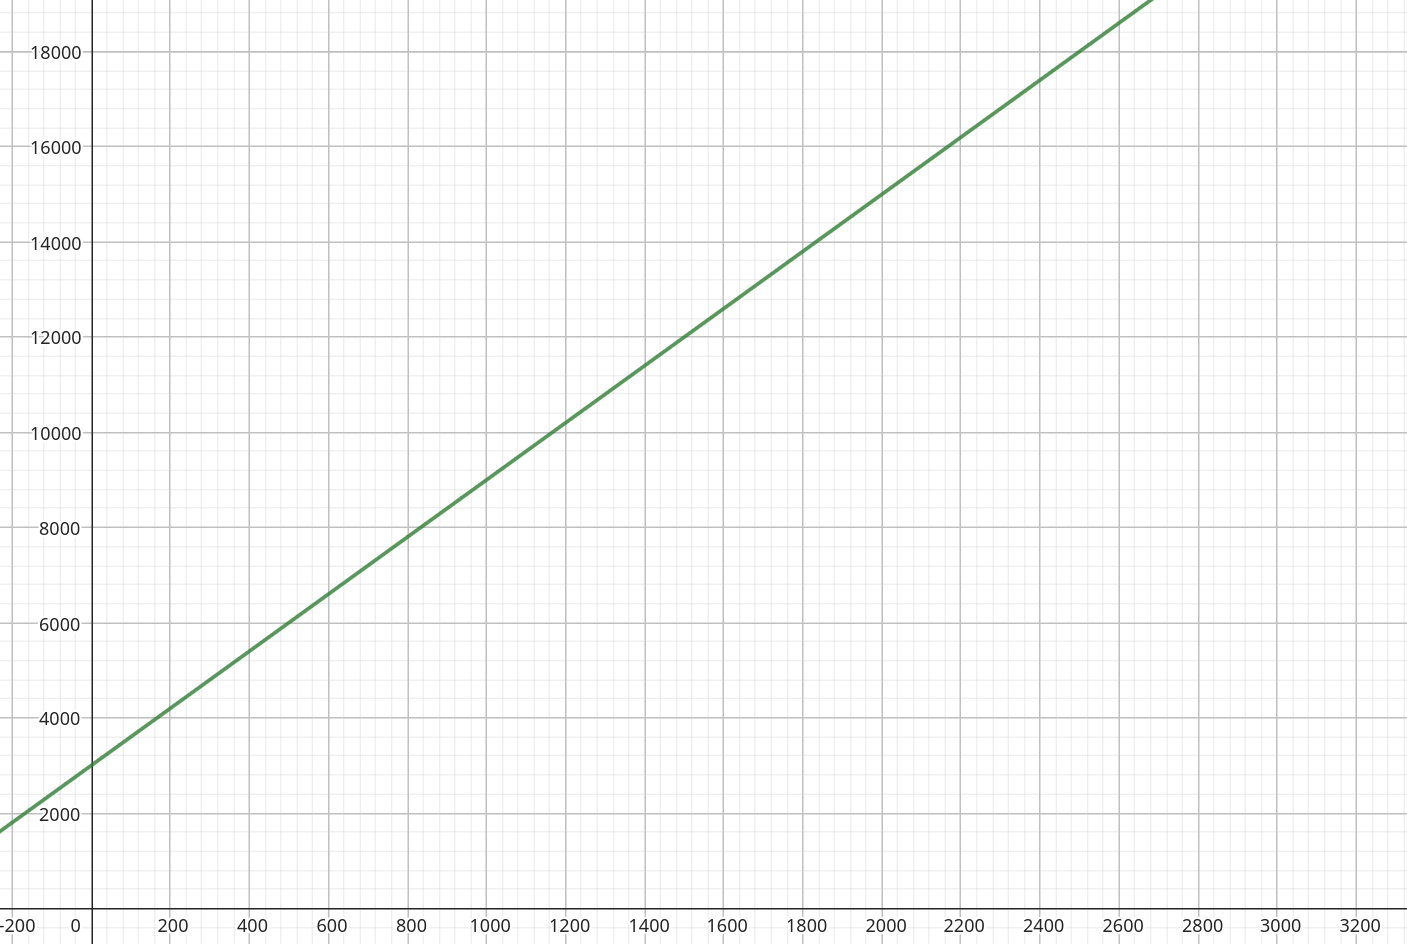
\includegraphics[width=10cm]{img/tostadoras.png}
\end{figure}

\item  ¿Cuál es la pendiente de la gráfica y qué representa?
\\ \\
La pendiente de la recta es $m=6$ y representa la razón de cambio, en este caso el aumento, del costo de producción en dólares respecto al número de tostadoras producidas. Esto significa que, agregar una tostadora implica subir el costo en 6 dólares.\\ 
 
\item  ¿Cuál es la intersección de la gráfica con el eje $y$ y qué representa?
\\
\[
f(0) = (6 \cdot 0) + 3000 = 3000
\]
La intersección con el eje $y$ es 3000 y representa el costo inicial de producción. No depende del número de tostadoras, es una constante sumada al costo independiente del número de tostadoras.
\\
\end{enumerate}

%sección 4
\section{Problema 27}
Zarco Romero José Antonio\\
\\
La población de ciertas especies en un ambiente limitado con una población inicial de 100 y capacidad para 1 000 es 
\[
P (t) = \frac{100 000}{100 + 900 e^{-t}} 
\]
donde t se mide en años.

\begin{enumerate}
\item Grafique esta función y estime cuánto tiempo le toma a la población llegar a 900.\\
\begin{figure}[h]
\centering
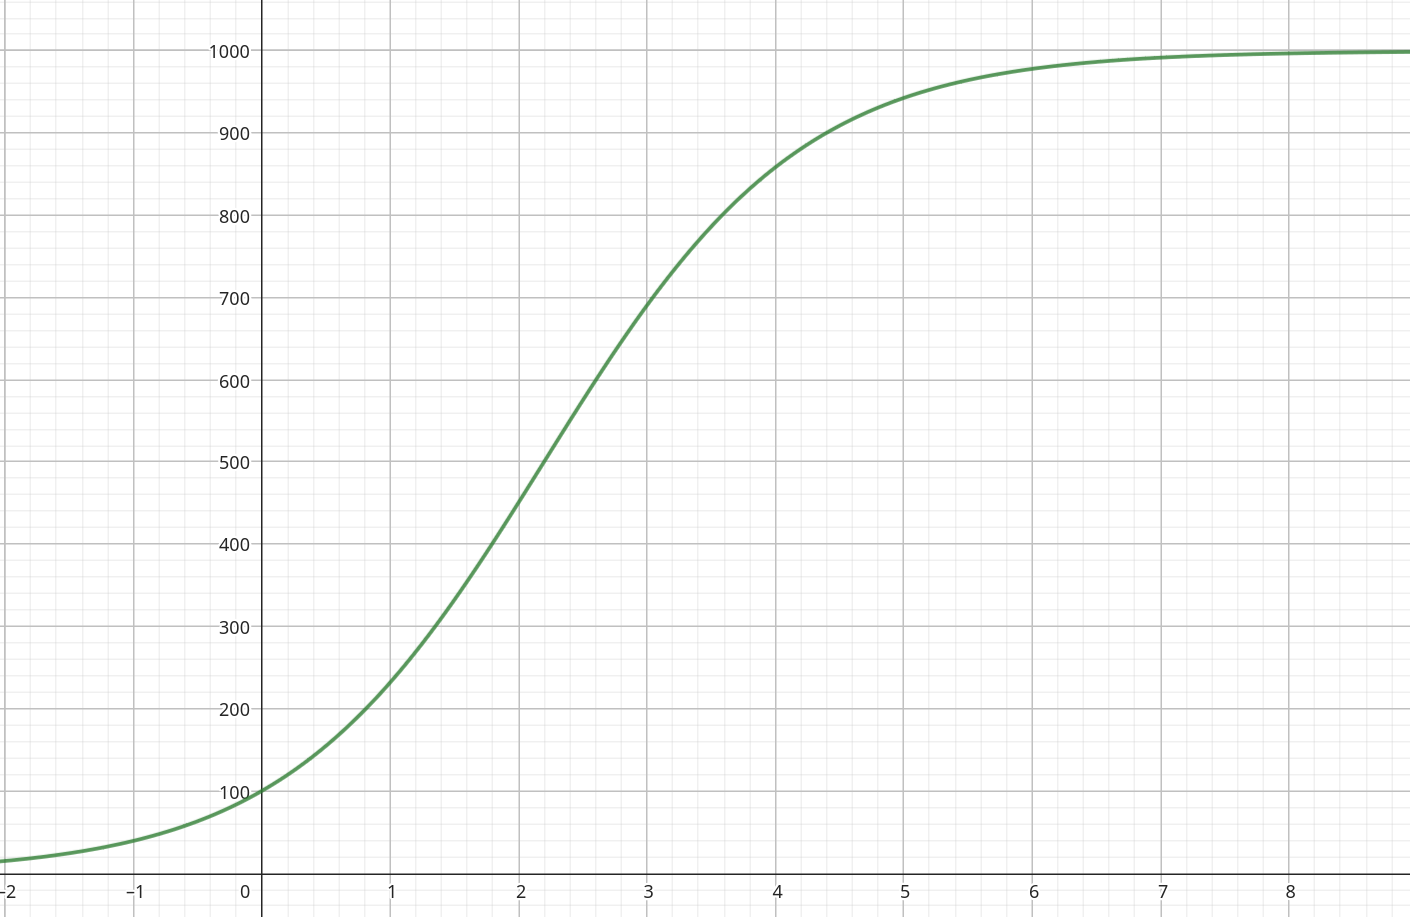
\includegraphics[ width=1\textwidth]{img/graficaPob.png}
\end{figure}
\\
Aprox 4.4 años. $P(4.4) = 900.4984$

\item Encuentre la inversa de esta función y explique su significado.
\[
P = \frac{100 000}{100 + 900 e^{-t}} 
\]
Para encontrar la función inversa, debemos despejar $t$ en términos de $P$
\[
 100 + 900 e^{-t}=\frac{100 000}{P}
\]
\[
e^{-t}=\frac{100 000- 100P}{900P}
\]
\[
t=-ln (\frac{100 000- 100P}{900P} )
\]
\[
\therefore t=-ln (\frac{1 000- P}{9P} )
\]

Entonces, la función inversa es
\[
P^{-1}(t)  = -ln (\frac{1 000 - t}{9t} )
\]
y representa el tiempo requerido  para que la población de ciertas especies alcance un número t.

\item Utilice la función inversa para encontrar el tiempo
necesario para que la población llegue a 900. Compare
con el resultado del inciso 1 \\

Usando la función inversa para encontrar el tiempo necesario para que la población alcance 900, obtenemos
\[
P(900) = -ln (\frac{1 000- 900}{9(900)} )=-ln(\frac{100}{8100})=-ln(\frac{1}{81})=-(ln1-ln81)
\]
\[
=ln81-ln1=ln81-0=ln(81) = 4.3944491546724 
\]
$\approx 4.4$ años.
\end{enumerate}


\end{document}